\documentclass{extbook}[14pt]
\usepackage{multicol, enumerate, enumitem, hyperref, color, soul, setspace, parskip, fancyhdr, amssymb, amsthm, amsmath, latexsym, units, mathtools}
\everymath{\displaystyle}
\usepackage[headsep=0.5cm,headheight=0cm, left=1 in,right= 1 in,top= 1 in,bottom= 1 in]{geometry}
\usepackage{dashrule}  % Package to use the command below to create lines between items
\newcommand{\litem}[1]{\item #1

\rule{\textwidth}{0.4pt}}
\pagestyle{fancy}
\lhead{}
\chead{Answer Key for Makeup Progress Quiz 2 Version C}
\rhead{}
\lfoot{2790-1423}
\cfoot{}
\rfoot{Summer C 2021}
\begin{document}
\textbf{This key should allow you to understand why you choose the option you did (beyond just getting a question right or wrong). \href{https://xronos.clas.ufl.edu/mac1105spring2020/courseDescriptionAndMisc/Exams/LearningFromResults}{More instructions on how to use this key can be found here}.}

\textbf{If you have a suggestion to make the keys better, \href{https://forms.gle/CZkbZmPbC9XALEE88}{please fill out the short survey here}.}

\textit{Note: This key is auto-generated and may contain issues and/or errors. The keys are reviewed after each exam to ensure grading is done accurately. If there are issues (like duplicate options), they are noted in the offline gradebook. The keys are a work-in-progress to give students as many resources to improve as possible.}

\rule{\textwidth}{0.4pt}

\begin{enumerate}\litem{
Choose the equation of the function graphed below.

\begin{center}
    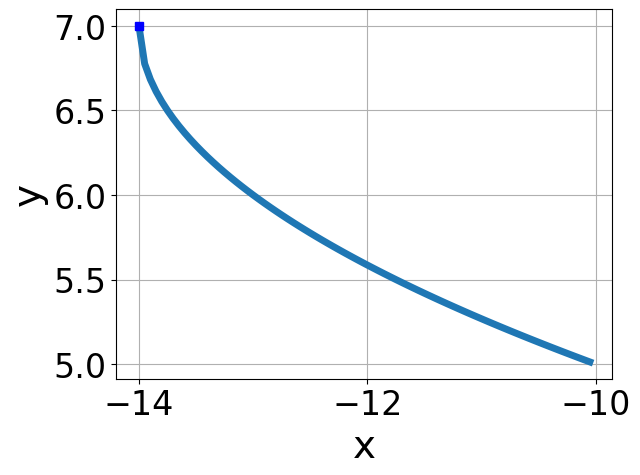
\includegraphics[width=0.5\textwidth]{../Figures/radicalGraphToEquationCopyC.png}
\end{center}


The solution is \( \text{None of the above} \), which is option E.\begin{enumerate}[label=\Alph*.]
\item \( f(x) = - \sqrt[3]{x + 14} + 7 \)

This would be the correct option if the root degree was $2$.
\item \( f(x) = \sqrt[3]{x + 14} + 7 \)

This corresponds to switching the coefficient and having the correct vertex with the root degree as $3$.
\item \( f(x) = \sqrt[3]{x - 14} + 7 \)

This corresponds to switching the coefficient AND switching the $x$-value of the vertex with the root degree as $3$.
\item \( f(x) = - \sqrt[3]{x - 14} + 7 \)

This corresponds to the correct coefficient and switching the $x$-value of the vertex with the root degree as $3$.
\item \( \text{None of the above} \)

* This is correct! The general shape of the graph is not correct for the radical power.
\end{enumerate}

\textbf{General Comment:} Remember that the general form of a radical equation is $ f(x) = a \sqrt[b]{x - h} + k$, where $a$ is the leading coefficient (and in this case, we assume is either $1$ or $-1$), $b$ is the root degree (in this case, either $2$ or $3$), and $(h, k)$ is the vertex.
}
\litem{
What is the domain of the function below?
\[ f(x) = \sqrt[8]{-7 x + 3} \]The solution is \( (-\infty, 0.429] \), which is option B.\begin{enumerate}[label=\Alph*.]
\item \( (-\infty, \infty) \)

This corresponds to the radical having an odd power, but the radical for this question is even.
\item \( (-\infty, a], \text{ where } a \in [0, 2] \)

* $(-\infty, 0.429]$, which is the correct option.
\item \( [a, \infty), \text{where } a \in [1.4, 5.4] \)

$[2.333, \infty)$, which corresponds to reversing the direction of the domain AND using the negative of the correct pivot value.
\item \( [a, \infty), \text{where } a \in [-1.9, 0.8] \)

 $[0.429, \infty)$, which corresponds to reversing the direction of the domain.
\item \( (-\infty, a], \text{where } a \in [1.8, 4.7] \)

$(-\infty, 2.333]$, which corresponds to using the negative of the correct pivot value.
\end{enumerate}

\textbf{General Comment:} Remember that we cannot take the even root of a negative number - this is why the domain is only sometimes restricted! If we have an even root, we solve $-7 x + 3 \geq 0$. Since this is an inequality, remember to flip the inequality if we divide by a negative number.
}
\litem{
Solve the radical equation below. Then, choose the interval(s) that the solution(s) belongs to.
\[ \sqrt{35 x^2 + 42} - \sqrt{-79 x} = 0 \]The solution is \( \text{that there are two solutions and they are } x = -1.400 \text{ and } x = -0.857. \), which is option E.\begin{enumerate}[label=\Alph*.]
\item \( x_1 \in [0.72, 1.71] \text{ and } x_2 \in [0.9,3.5] \)

$x = 0.857 \text{ and } x = 1.400$, which are the negative or absolute values of the values you would have gotten by solving the equation correctly.
\item \( \text{All solutions lead to invalid or complex values in the equation.} \)

Corresponds to thinking that $x = -1.400 \text{ and } x = -0.857$ lead to negatives in at least one of the radicands.
\item \( x \in [-1.61,-0.88] \)

$x = -1.400$, which corresponds to thinking that $x = -0.857$ leads to a negative in at least one of the radicands.
\item \( x \in [-0.88,-0.84] \)

$x = -0.857$, which corresponds to thinking that $x = -1.400$ leads to a negative in at least one of the radicands.
\item \( x_1 \in [-1.61, -0.88] \text{ and } x_2 \in [-1.2,0.3] \)

* $x = -1.400 \text{ and } x = -0.857$, which is the correct option.
\end{enumerate}

\textbf{General Comment:} Distractors are different based on the number of solutions. For example, if the question is designed to have 0 options, then the distractors are solving the equation and not checking that the solutions lead to complex numbers (because plugging them in makes the value under the square root negative). Remember that after solving, we need to make sure our solution does not make the original equation take the square root of a negative number!
}
\litem{
Choose the graph of the equation below.
\[ f(x) = - \sqrt{x - 6} + 7 \]The solution is the graph below, which is option B.
    \begin{center}
        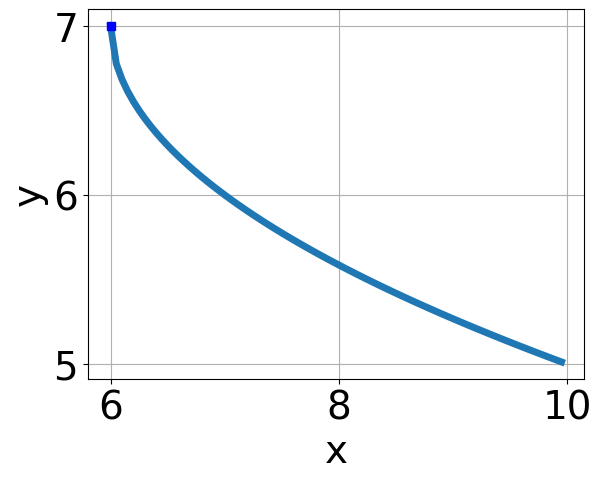
\includegraphics[width=0.3\textwidth]{../Figures/radicalEquationToGraphBC.png}
    \end{center}\begin{enumerate}[label=\Alph*.]
\begin{multicols}{2}
\item 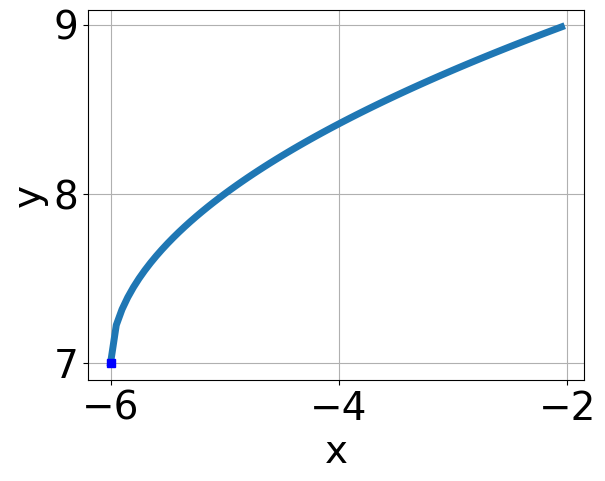
\includegraphics[width = 0.3\textwidth]{../Figures/radicalEquationToGraphAC.png}
\item 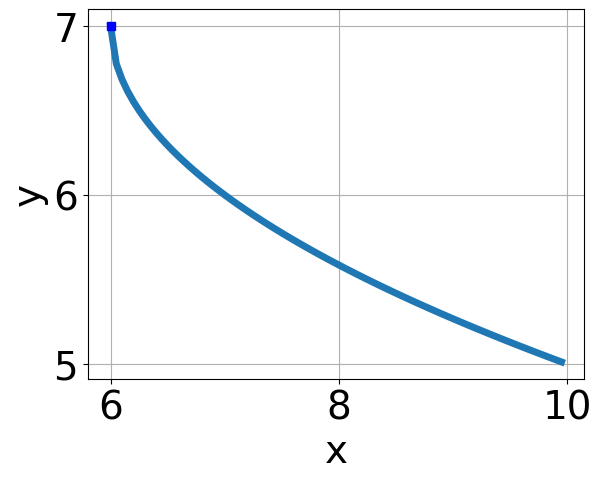
\includegraphics[width = 0.3\textwidth]{../Figures/radicalEquationToGraphBC.png}
\item 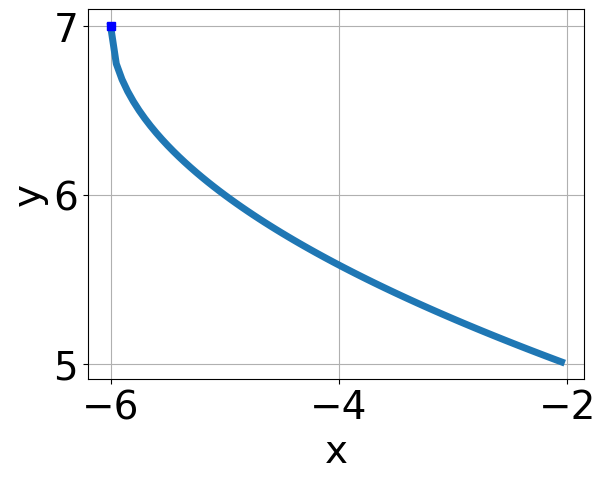
\includegraphics[width = 0.3\textwidth]{../Figures/radicalEquationToGraphCC.png}
\item 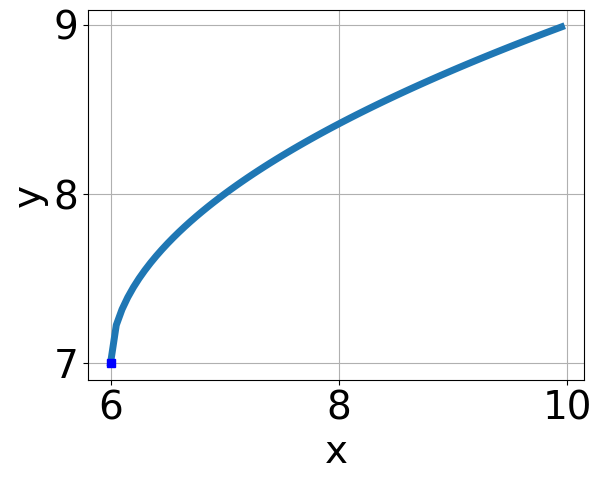
\includegraphics[width = 0.3\textwidth]{../Figures/radicalEquationToGraphDC.png}
\end{multicols}\item None of the above.\end{enumerate}
\textbf{General Comment:} Remember that the general form of a radical equation is $ f(x) = a \sqrt[b]{x - h} + k $, where $a$ is the leading coefficient (and in this case, we assume is either 1 or -1), $b$ is the root degree (in this case, either 2 or 3), and $(h, k)$ is the vertex.
}
\litem{
What is the domain of the function below?
\[ f(x) = \sqrt[4]{6 x - 4} \]The solution is \( [0.667, \infty) \), which is option A.\begin{enumerate}[label=\Alph*.]
\item \( [a, \infty), \text{ where } a \in [0.51, 1.35] \)

* $[0.667, \infty)$, which is the correct option.
\item \( [a, \infty), \text{where } a \in [1.46, 1.7] \)

$[1.500, \infty)$, which corresponds to using the negative of the correct pivot value.
\item \( (-\infty, a], \text{where } a \in [1.3, 4.3] \)

$(-\infty, 1.500]$, which corresponds to reversing the direction of the domain AND using the negative of the correct pivot value.
\item \( (-\infty, \infty) \)

This corresponds to the radical having an odd power, but the radical for this question is even.
\item \( (-\infty, a], \text{where } a \in [0.5, 1] \)

 $(-\infty, 0.667]$, which corresponds to reversing the direction of the domain.
\end{enumerate}

\textbf{General Comment:} Remember that we cannot take the even root of a negative number - this is why the domain is only sometimes restricted! If we have an even root, we solve $6 x - 4 \geq 0$. Since this is an inequality, remember to flip the inequality if we divide by a negative number.
}
\litem{
Solve the radical equation below. Then, choose the interval(s) that the solution(s) belongs to.
\[ \sqrt{-6 x - 5} - \sqrt{2 x + 5} = 0 \]The solution is \( x = -1.25 \), which is option C.\begin{enumerate}[label=\Alph*.]
\item \( x_1 \in [-2.6, -1.5] \text{ and } x_2 \in [-5.83,1.17] \)

$x = -2.500$ and $x = -0.833$, which corresponds to solving each radical separately for 0.
\item \( x \in [-0.7,1.3] \)

$x = -0.000$, which corresponds to squaring each square root separately and assigning the negative to the third term.
\item \( x \in [-2.1,-0.4] \)

* $x = -1.250$, which is the correct option.
\item \( x_1 \in [-2.1, -0.4] \text{ and } x_2 \in [-5.83,1.17] \)

$x = -1.250$ and $x = -0.833$, which corresponds to solving the equation correctly and including the value that makes the first square root 0.
\item \( \text{All solutions lead to invalid or complex values in the equation.} \)

This corresponds to believing the solution $x = -1.250$ leads to a complex value in the original equation.
\end{enumerate}

\textbf{General Comment:} Distractors are different based on the number of solutions. For example, if the question is designed to have 0 options, then the distractors are solving the equation and not checking that the solution leads to complex numbers (because plugging them in makes the value under the square root negative). Remember that after solving, we need to make sure our solution does not make the original equation take the square root of a negative number!
}
\litem{
Choose the equation of the function graphed below.

\begin{center}
    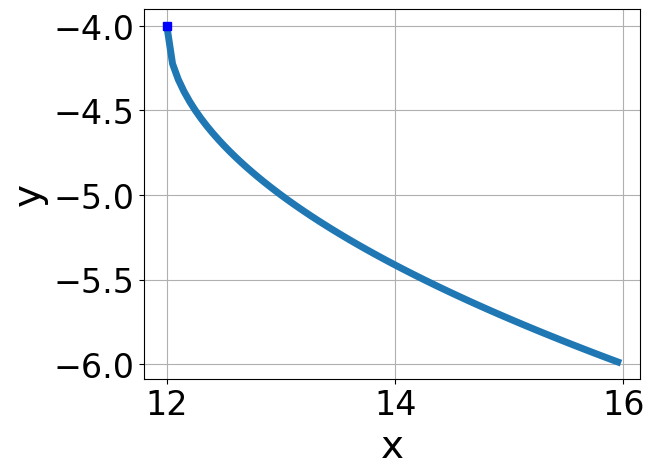
\includegraphics[width=0.5\textwidth]{../Figures/radicalGraphToEquationC.png}
\end{center}


The solution is \( - \sqrt{x - 12} - 4 \), which is option D.\begin{enumerate}[label=\Alph*.]
\item \( f(x) = \sqrt{x + 12} - 4 \)

This corresponds to switching the coefficient AND switching the $x$-value of the vertex with the root degree as $2$.
\item \( f(x) = - \sqrt{x + 12} - 4 \)

This corresponds to the correct coefficient and switching the $x$-value of the vertex with the root degree as $2$.
\item \( f(x) = \sqrt{x - 12} - 4 \)

This corresponds to switching the coefficient and having the correct vertex with the root degree as $2$.
\item \( f(x) = - \sqrt{x - 12} - 4 \)

* This is the correct option.
\item \( \text{None of the above} \)

You likely though the graphs did not match the power of the radical.
\end{enumerate}

\textbf{General Comment:} Remember that the general form of a radical equation is $ f(x) = a \sqrt[b]{x - h} + k$, where $a$ is the leading coefficient (and in this case, we assume is either $1$ or $-1$), $b$ is the root degree (in this case, either $2$ or $3$), and $(h, k)$ is the vertex.
}
\litem{
Solve the radical equation below. Then, choose the interval(s) that the solution(s) belongs to.
\[ \sqrt{-9 x^2 - 24} - \sqrt{33 x} = 0 \]The solution is \( \text{all potential solutions lead to complex values in the equation.} \), which is option E.\begin{enumerate}[label=\Alph*.]
\item \( x_1 \in [2.58, 3.03] \text{ and } x_2 \in [-0.1,4.2] \)

$x = 2.667 \text{ and } x = 1.000$, which corresponds to getting the negatives of the values that make the equation 0.
\item \( x \in [-2.44,-0.68] \)

$x = -1.000$, which corresponds to not checking that this value makes at least one of the radicands negative.
\item \( x \in [-3.14,-2.26] \)

$x = -2.667$, which corresponds to not checking that this value makes at least one of the radicands negative.
\item \( x_1 \in [-3.14, -2.26] \text{ and } x_2 \in [-1.4,0.9] \)

$x = -2.667 \text{ and } x = -1.000$, which corresponds to not checking that BOTH values make at least one of the radicands negative.
\item \( \text{All solutions lead to invalid or complex values in the equation.} \)

* This is the correct option.
\end{enumerate}

\textbf{General Comment:} Distractors are different based on the number of solutions. For example, if the question is designed to have 0 options, then the distractors are solving the equation and not checking that the solutions lead to complex numbers (because plugging them in makes the value under the square root negative). Remember that after solving, we need to make sure our solution does not make the original equation take the square root of a negative number!
}
\litem{
Choose the graph of the equation below.
\[ f(x) = - \sqrt{x - 12} + 7 \]The solution is the graph below, which is option D.
    \begin{center}
        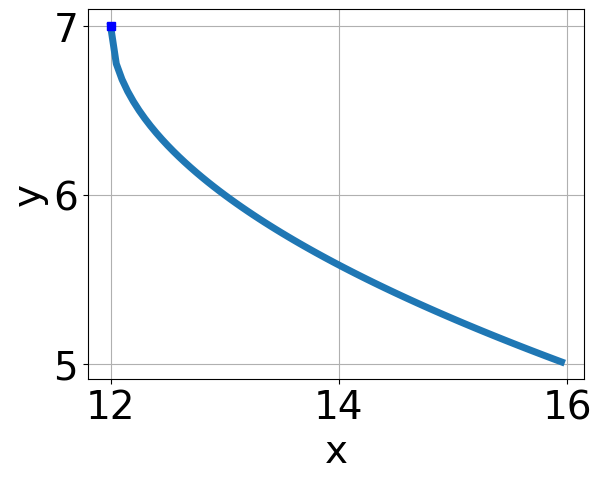
\includegraphics[width=0.3\textwidth]{../Figures/radicalEquationToGraphCopyDC.png}
    \end{center}\begin{enumerate}[label=\Alph*.]
\begin{multicols}{2}
\item 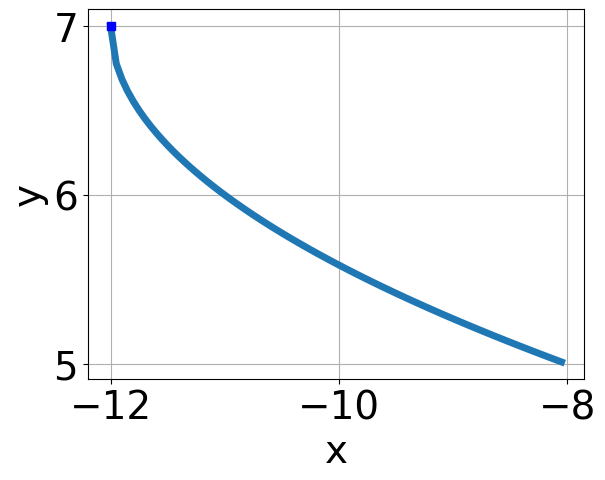
\includegraphics[width = 0.3\textwidth]{../Figures/radicalEquationToGraphCopyAC.png}
\item 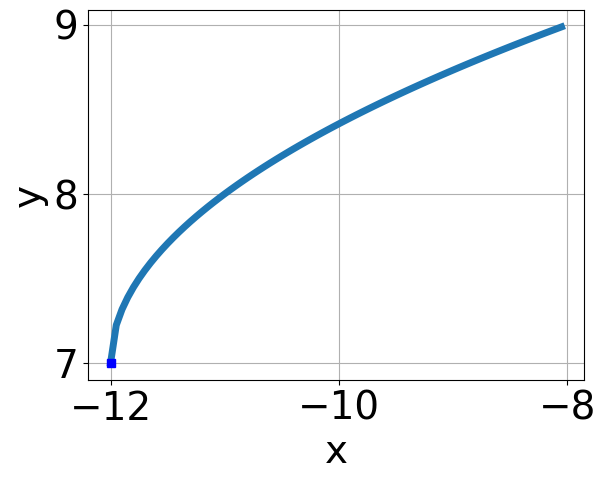
\includegraphics[width = 0.3\textwidth]{../Figures/radicalEquationToGraphCopyBC.png}
\item 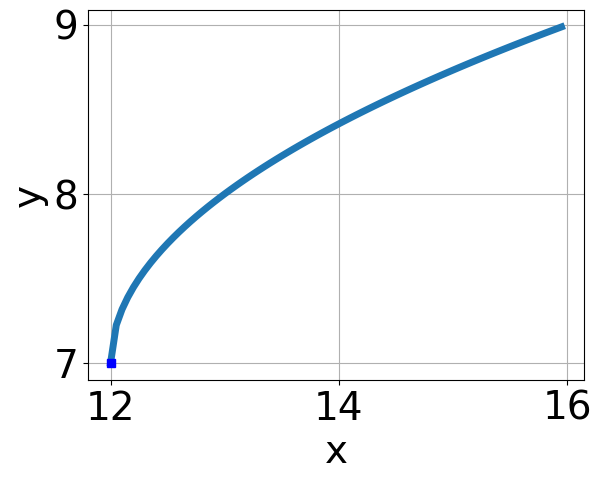
\includegraphics[width = 0.3\textwidth]{../Figures/radicalEquationToGraphCopyCC.png}
\item 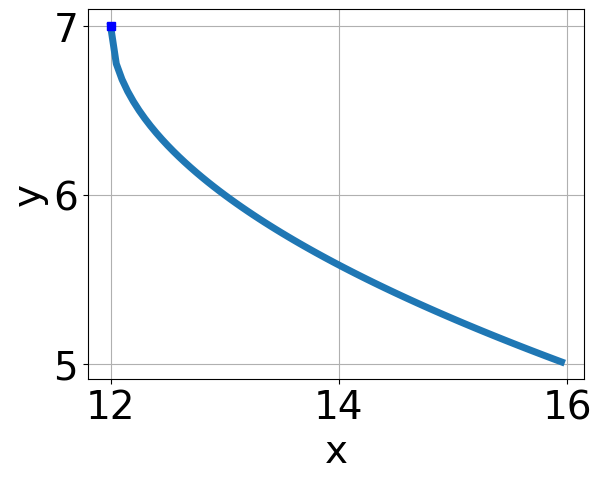
\includegraphics[width = 0.3\textwidth]{../Figures/radicalEquationToGraphCopyDC.png}
\end{multicols}\item None of the above.\end{enumerate}
\textbf{General Comment:} Remember that the general form of a radical equation is $ f(x) = a \sqrt[b]{x - h} + k $, where $a$ is the leading coefficient (and in this case, we assume is either 1 or -1), $b$ is the root degree (in this case, either 2 or 3), and $(h, k)$ is the vertex.
}
\litem{
Solve the radical equation below. Then, choose the interval(s) that the solution(s) belongs to.
\[ \sqrt{4 x - 6} - \sqrt{7 x - 4} = 0 \]The solution is \( \text{All solutions lead to invalid or complex values in the equation.} \), which is option D.\begin{enumerate}[label=\Alph*.]
\item \( x_1 \in [-1.08, 0.01] \text{ and } x_2 \in [1.5,3.5] \)

$x = -0.667$ and $x = 1.500$, which corresponds to solving the equation correctly and including the value that makes the first square root 0.
\item \( x \in [-1.08,0.01] \)

This corresponds to not checking that the potential solution $x = -0.667$ leads to a complex value in the original equation.
\item \( x \in [-3.64,-3.28] \)

$x = -3.333$, which corresponds to squaring each square root separately and assigning the negative to the third term.
\item \( \text{All solutions lead to invalid or complex values in the equation.} \)

*$x = -0.667$ leads to a complex value in the equation, so this is the correct option.
\item \( x_1 \in [-0.51, 0.84] \text{ and } x_2 \in [1.5,3.5] \)

$x = 0.571$ and $x = 1.500$, which corresponds to solving each radical separately for 0.
\end{enumerate}

\textbf{General Comment:} Distractors are different based on the number of solutions. For example, if the question is designed to have 0 options, then the distractors are solving the equation and not checking that the solution leads to complex numbers (because plugging them in makes the value under the square root negative). Remember that after solving, we need to make sure our solution does not make the original equation take the square root of a negative number!
}
\end{enumerate}

\end{document}